\marginpar{VL am 20.05.19}
\subsubsection{Algebraische Netzbeschreibung}
Basis für die PN-Darstellung in Rechner und die PN-Analyse(s. Kapitel 4).

\underline{Begriffe:} \beiblatt{2-11, 2-12}

\properparagraph{Beispiel}

\begin{figure}[H]
	\centering
	\includegraphics[width=5cm]{img/2019_05_20/abb1.tikz}
\end{figure}

\begin{subequations}
	\begin{align}
	\ubar{K}   &= \begin{bmatrix}10\\2\end{bmatrix} \\
	\ubar{t}_1 &= \begin{bmatrix}3\\-1\end{bmatrix}\\
	\ubar{t}_2 &= \begin{bmatrix}-1\\2\end{bmatrix}\\
	\ubar{N}   &= \begin{bmatrix}t_1 & t_2\end{bmatrix} = \begin{bmatrix}3 & -1 \\ -1 & 2\end{bmatrix}\\
	\ubar{m}_0 &= \begin{bmatrix}1 \\ 0\end{bmatrix}
	\end{align}
\end{subequations}

Schaltvoraussetzung:
\begin{subequations}
	\begin{align}
	t_1 &: 0 \le \underbrace{\m{1\\0}+\m{3\\-1}}_{\m{4\\-1}} \le \m{10\\2}\\[2ex]
	t_2 &: 0 \le \underbrace{\m{1\\0}+\m{1\\2}}_{\m{0\\2}} \le \m{10\\2}
	\end{align}
\end{subequations}

Schaltvektor: $t_2$ aktiviert $\Rightarrow \ubar{v}(1)=\m{0\\1}$

Folgemarkierung: $\ubar{m}(1)=\ubar{m}(0) + \ubar{N} \ubar{v}(1) = \m{1\\0}+\m{3&-1\\-1&2} \m{0\\1} = \m{0\\2}$

(weitere Schaltvorgänge analog)

\subsubsection{Darstellung von Nebenläufigkeit}
Untersuchung der Modellierungstransparenz bei Nebenläufigkeiten: PN $\leftrightarrow$ Automat.

\properparagraph{Beispiel: Zwei Prozesse}

\begin{tabular}{l|l|l}
	 & Zustände & Ereignisse \\
	 \hline
	 $P_1$ & $z_1,z_2,z_3$ & $e_1,e_2,e_3$ \\
	 \hline
	 $P_2$ & $z_4,z_5,z_6$ & $e_4,e_5,e_6$ 
\end{tabular}

Nebenläufigkeiten: 
\begin{itemize}
	\item asynchron: Ereignisse treten unabhängig voneinander auf
	\item hier: $e_3$ und $e_6$ treten gleichzeitig auf
\end{itemize}

Vergleich: lokaler(getrennter) und globaler Automatengraph mit PNen (s. BB AEH 2-13)

Fazit: PN aufgrund der verteilten Zustandsinformation (Markierung) und den transparenten Strukturen (bei synchronisierten Nebenläufigkeiten) kompakter und übersichtlicher.

\subsubsection{Zeitbewertung}
Bei PN erforderlich, falls neben kausalen Ablauf auch zeitlicher Zusammenhang relevant. 

Prinzip: \beiblatt{2-14}\\
(Sonderfall: Ereignisse nicht zeitbewertet: $\tau_R=0$, $\tau_L=\infty$)

\properparagraph{Beispiel: Kleben von Teilen}

\begin{figure}[H]
	\centering
	\includegraphics[]{img/2019_05_20/abb3.tikz}
\end{figure}

Weitere Beispiele \beiblatt{2-15}

\subsubsection{Test- und Inhibitorkanten}
Spezielle Kanten zur Einbringung zusätzlicher Bedingungen in die Dynamik ohne Markenfluss beim Schaltvorgang \beiblatt{2-16}

\properparagraph{Beispiel: Synchronisation ansonsten unabhängiger Prozesse} 
\begin{figure}[H]
	\centering
	\includegraphics[]{img/2019_05_20/abb4.tikz}
\end{figure}

$t_4$ immer erst nach dem Schalten von $t_3$ und $t_2$ aktiviert.

Vorteil: Übersichtliche Darstellung\\
Nachteil: Analyse erschwert

\includepdf[pages={21 - 26}]{material/AEH_2019.pdf}

\subsection{Netz - Condition/Event - Systeme}
\underline{PN-Schwächen:}
\begin{itemize}
	\item Kein Ein-/Ausgangsgrößenkonzept
	\item Komplizierte Modularisierung
\end{itemize}

\underline{Abhilfe:} Netz Condition/Event (NCE) Systeme

\subsubsection{Signalkonzepte bei CE-Systemen}
\underline{Condition/Event (CE)-Systeme} (1991)
Konzept zur transparenten Kopplung von DES-Modellen über zwei spezielle Signaltypen:
\begin{itemize}
	\item \textbf{Conditionsignale:} liefern (als stückweise konstante Funktionen) Informationen über aktuelle Zustände im zugehörigen Modul, die als Bedingung Ereignisse in anderen Modulen ermöglichen bzw. verhindern.
	
	\begin{figure}[H]
		\centering
		\includegraphics[width=0.5\textwidth]{img/2019_05_20/abb5.tikz}
	\end{figure}

	Signalflussbild: \begin{tikzpicture}\draw[-Stealth] (0,0) -- (2,0);\end{tikzpicture} (auch: \begin{tikzpicture}\draw[-Stealth] (0,0) -- (2,0);\draw[fill] (0.8,-0.07) rectangle (1,0);\draw[fill] (1,0) rectangle (1.2,0.07);\end{tikzpicture})
	
	\item \textbf{Eventsignale:} Liefern als zeitdiskrete Impulse Informationen über aktuell stattfindende Ereignisse im zugehörigen Modul, die Ereignisse in anderen Modulen erzwingen.
	
	\begin{figure}[H]
		\centering
		\includegraphics[width=0.5\textwidth]{img/2019_05_20/abb7.tikz}
	\end{figure}

	Signalflussbild: \begin{tikzpicture}\draw[-Stealth] (0,0) -- (0.90,0) -- (0.95,0.1) -- (1.05,-0.1) -- (1.1,0) -- (2,0);\end{tikzpicture}
	
	Blockschaltbild eines Moduls:
	\begin{figure}[H]
		\centering
		\includegraphics[]{img/2019_05_20/abb8.tikz}
	\end{figure}

	hier: DES-Modellierung im Modul als PN $\Rightarrow$ Netz-Condition/Event-Systeme (NCE)
	(im Prinzip aber beliebig, auch z.B. Automaten eingesetzt)
	 
\end{itemize}